\documentclass[a4paper]{report}
\usepackage{titlesec}
\usepackage{pdfpages}
\usepackage{fancyhdr}
\usepackage[hyphens]{url}
\usepackage{hyperref}
\hypersetup{
  colorlinks=true,
  linkcolor=blue,
  filecolor=magenta,
  urlcolor=cyan,
}
\urlstyle{same}


\newcommand{\mytitle}{Course Pack: Meaningful Text Analysis with Word Embeddings}

\pagestyle{headings}

\title{Course Pack: Meaningful Text Analysis with Word Embeddings, Digital Humanities Summer Institute, 2022}
\author{Jonathan Reeve}
\date{June, 2022}

\begin{document}

\maketitle

\tableofcontents

\chapter{About this Course Pack}

This course pack contains a syllabus and readings that may be of interest to students in the course, ``Meaningful Text Analysis with Word Embeddings,'' a one-week course at the Digital Humanities Summer Institute, during the summer of 2022. Many of the readings are meant for a technical audience, so you may encounter notation or terminology that will seem unfamiliar. Please don't let that discourage you! In this course, we will not need most of the mathematical details you see in these papers, since we will be using libraries and software packages that have already implemented these details for us. That said, if you're curious about the inner workings of the algorithms we'll be using, or have a background in computer science, those details can be useful!

The first of these readings is from the classic textbook from Jurafski and Martin, \emph{Speech and Language Processing}. Following that is Mikolov et al's seminal paper describing Word2Vec, one of the most well-known embedding libraries. Finally, there are papers which deal with humanities applications, and potential ethics issues associated with word embeddings analysis.

Find all these readings, and more, at the course website: \url{https://dhsi2022.jonreeve.com}, which is the canonical location for course materials.

%% \chapter{Jurafsky's Slides}

%% Slides for Chapter 6 of Jurafski, Dan, and James H. Martin. \emph{Speech and Language Processing}. Third edition draft. \url{https://web.stanford.edu/~jurafsky/slp3/}

%%   %% \includepdf[pagecommand={\thispagestyle{empty}},pages=1 ]{jurafsky2020.pdf}
%%   \includepdf[pagecommand={\thispagestyle{headings}}, pages=1-]{jurafsky2020.pdf}

\chapter{Syllabus}

NB: This syllabus is subject to some change. The most up-to-date version of this document may be found at \url{https://dhsi2022.jonreeve.com/}.

\section{Course Description}

Word embeddings provide new ways of understanding language, by encorporating contexts, meanings, and senses of words into their digital representations. They are a new technology, developed by researchers at Google, which now powers the most advanced computational language tasks, such as machine translation, automatic summarization, and information extraction. Since they represent more than just the surface forms of words, their applications for humanities scholarship are profound. This course will serve as a hands-on introduction to word embeddings, and will use the Python programming language, in conjunction with the SpaCy package for natural language processing. Participants are encouraged to bring their own collections of text to analyze, and will create meaningful explorations of them by the end of the course. No prior programming experience is necessary.

\section{Course Information}

\begin{itemize}
\item \textbf{Instructor}: Jonathan Reeve, Department of English and Comparative Literature, Columbia University.
\item \textbf{Instructor email address}: jonathan.reeve@columbia.edu
\item \textbf{Course website}: \url{http://dhsi2022.jonreeve.com/}
\item \textbf{Dates}: 6–10 June, 2022
\item \textbf{Videoconference link}: \url{https://meet.jit.si/dhsi2022-word-embeddings}.
\item \textbf{Chatroom}: \#dhsi2022-word-embeddings on Matrix
\end{itemize}

\section{Schedule}

Each day I'll post a lecture video to the course website, usually around one hour in length. Please watch the lecture videos before coming to class, and follow along on your own computer. Class sessions will be held over videoconference, at \url{https://meet.jit.si/dhsi2022-word-embeddings}. For more details, please visit the course website, \url{http://dhsi2022.jonreeve.com/}.

\begin{itemize}
  \item Monday, 6 June 2022. Introduction to the theory of word embeddings and word vectors. Reading: Jurafsky et al.
  \item Tuesday, 7 June 2022. Introduction to Python and SpaCy. Reading: Mikolov et al.
  \item Wednesday, 8 June 2022. Exploring pre-trained vector spaces. GloVe vectors. Reading: Kozlowski et al.
  \item Thursday, 9 June 2022. Text analysis with word embeddings. Reading: Garg et al.
  \item Friday, 10 June 2022. Collaborative lab work. Reading: Schiebinger, et al.
\end{itemize}

\chapter{Reading 1: Jurafsky}

Text of Chapter 6 of Jurafski, Dan, and James H. Martin. \emph{Speech and Language Processing}. Third edition draft. \url{https://web.stanford.edu/~jurafsky/slp3/}

  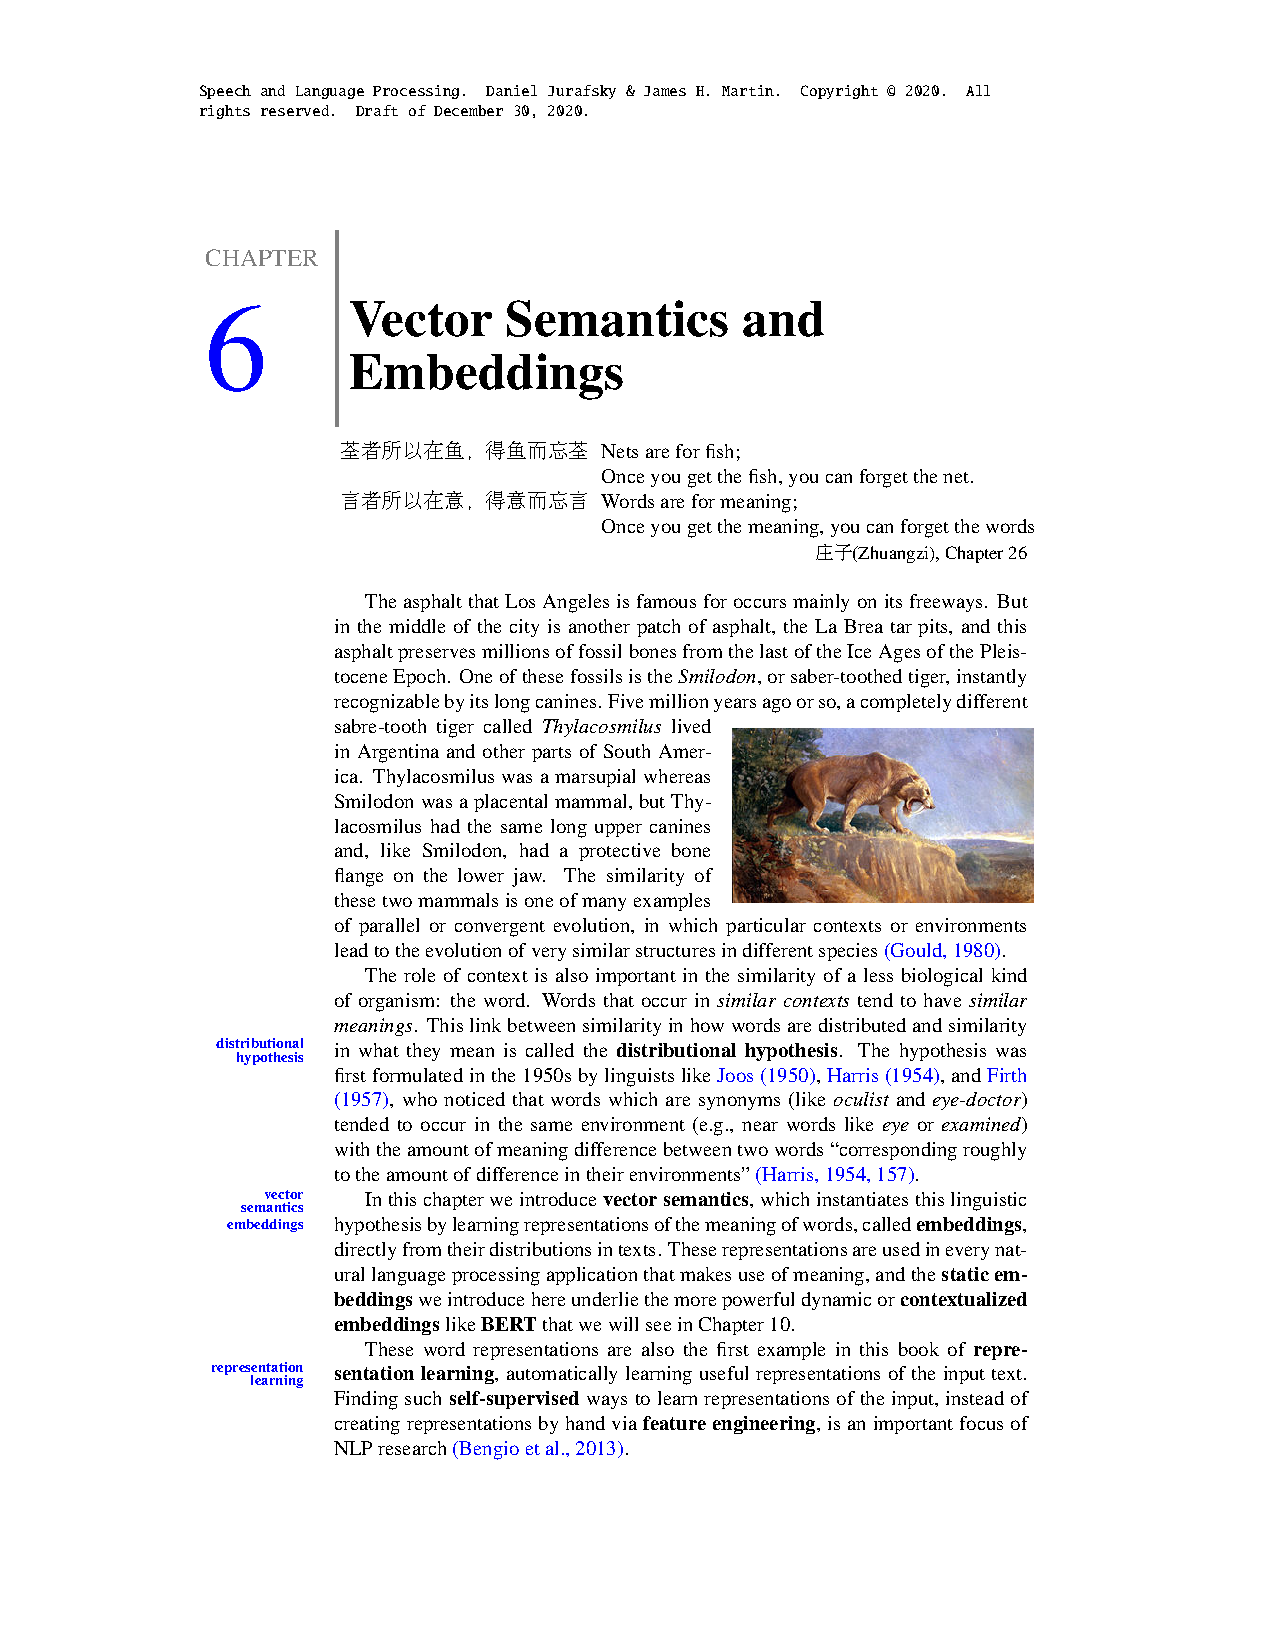
\includepdf[pagecommand={\thispagestyle{headings}}, pages=1-]{../content/static/readings/jurafsky.pdf}

\chapter{Reading 2: Mikolov et al.}

Mikolov, Tomas and Chen, Kai and Corrado, Greg and Dean, Jeffrey. ``Efficient estimation of word representations in vector space.'' arXiv preprint arXiv:1301.3781. https://arxiv.org/abs/1301.3781

  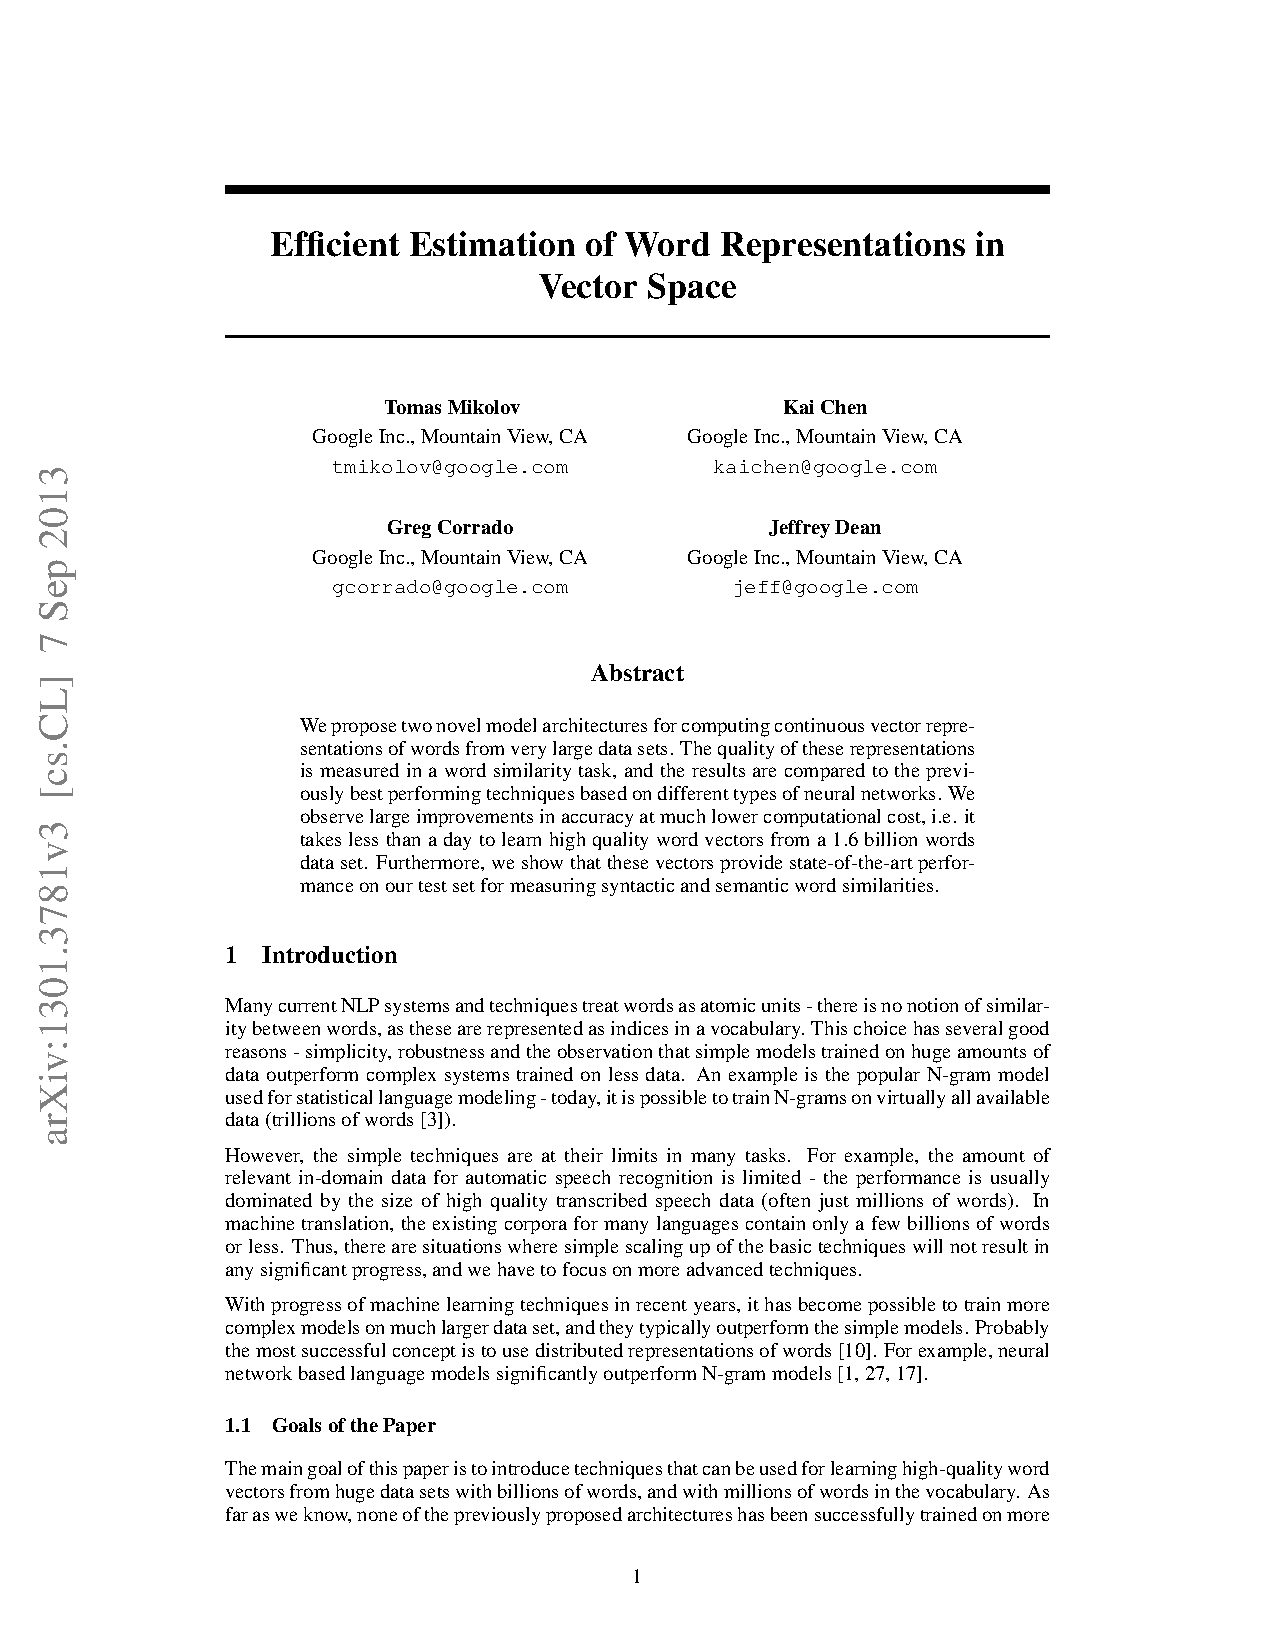
\includepdf[pagecommand={\thispagestyle{headings}}, pages=1-]{../content/static/readings/mikolov.pdf}

\chapter{Reading 3: Kozlowski et al.}

Kozlowski, Austin C., Matt Taddy, and Evans, James A. (2019) ``The Geometry of Culture: Analyzing the Meanings of Class through Word Embeddings''. American Sociological Review 84:5.

  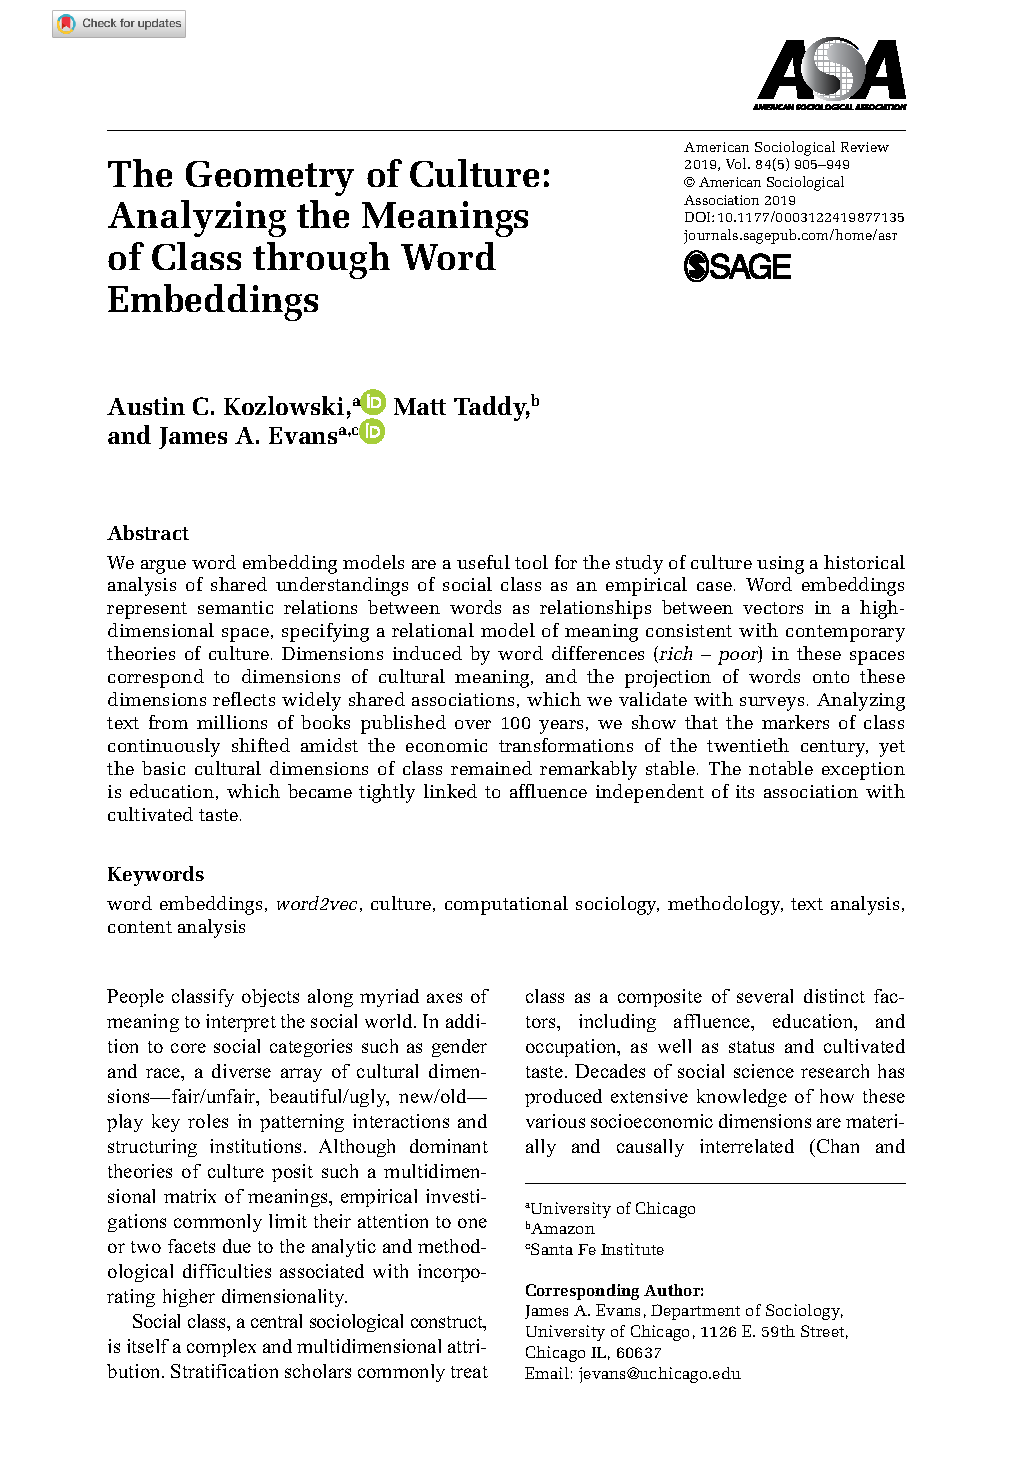
\includepdf[pagecommand={\thispagestyle{empty}}, pages=1-]{../content/static/readings/kozlowski.pdf}

\chapter{Reading 4: Garg et al.}

Garg, N., Schiebinger, L., Jurafsky, D., and Zou, J. (2018) ``Word embeddings quantify 100 years of gender and ethnic stereotypes'' PNAS 115:16.

  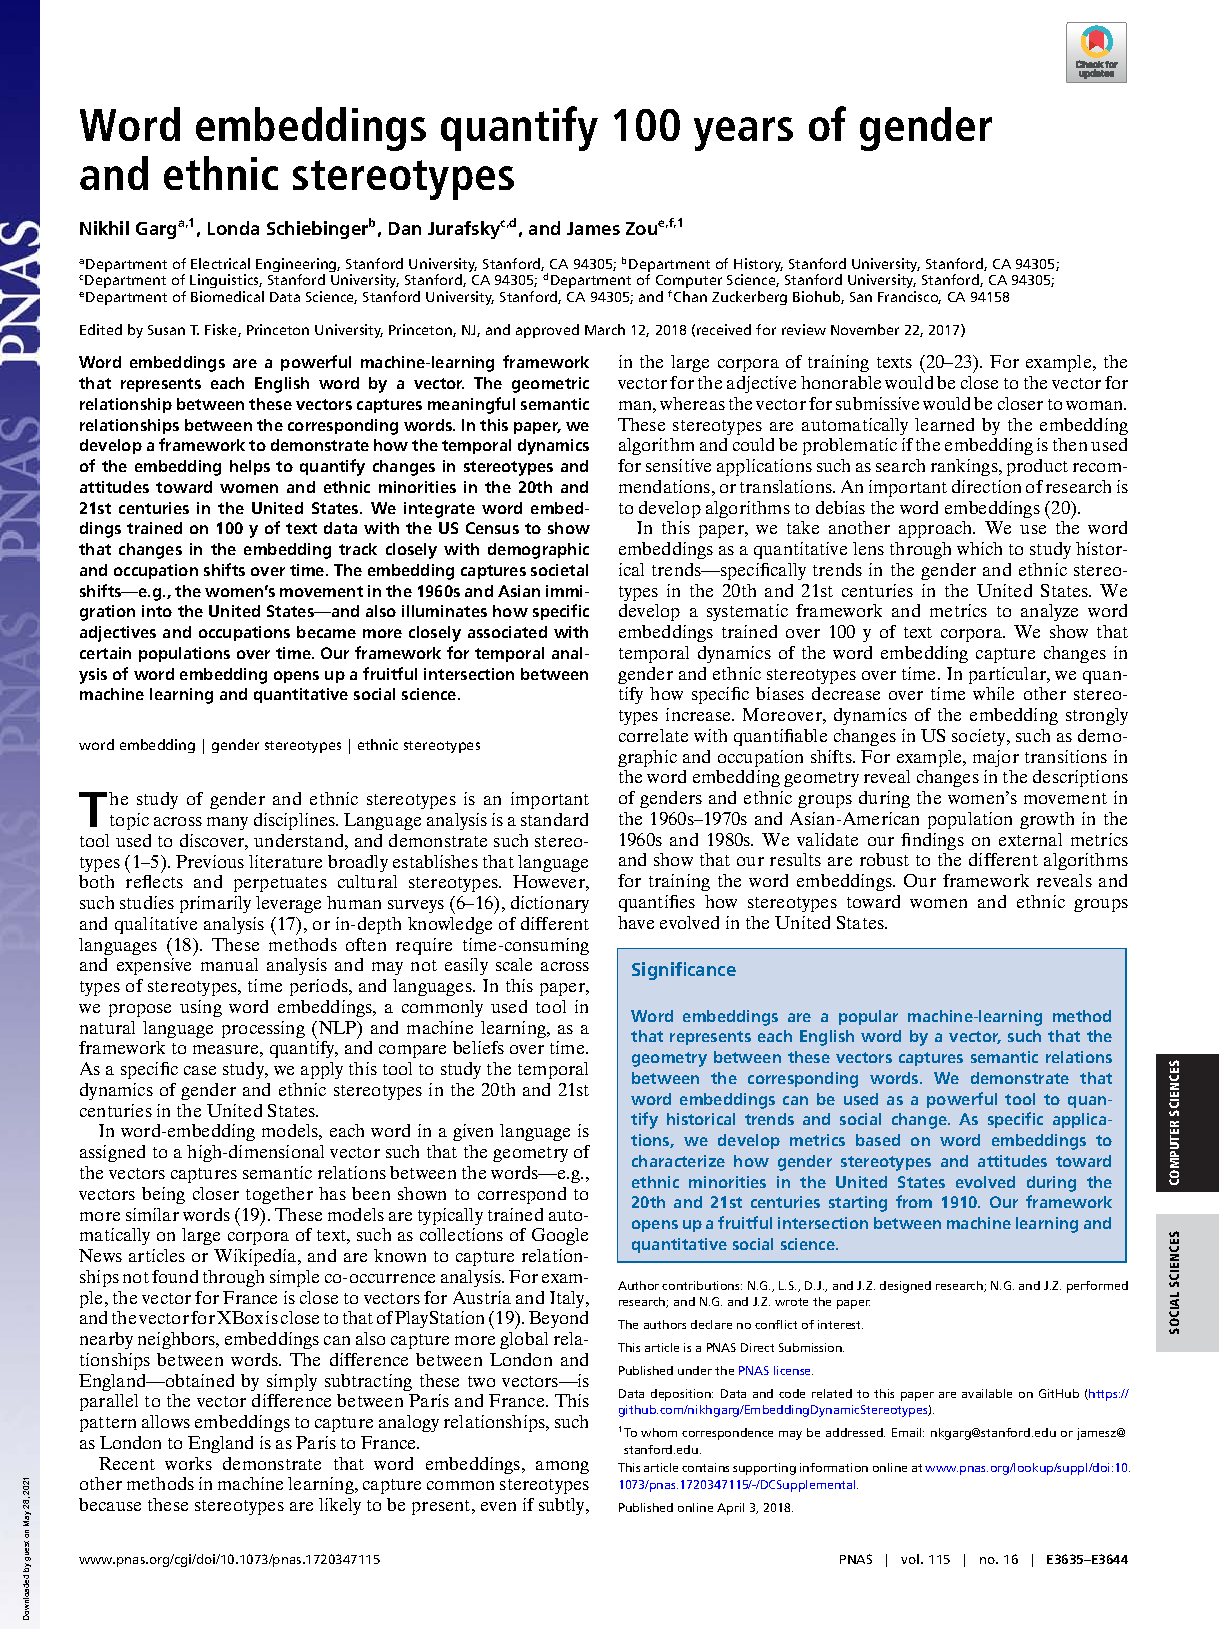
\includepdf[pagecommand={\thispagestyle{empty}}, pages=1-]{../content/static/readings/garg.pdf}

\end{document}
